\section{Implementation}

\lstset{
  columns=fixed,
  style=julia,
  escapechar=\%,
}

\subsection{DifferentialRiccatiEquations.jl}
\begin{frame}[label=code_dre]{\secname}
\framesubtitle{User Interface of \subsecname}
\only<+>{\lstinputlisting[lastline=18]{code/standalone_dre.jl.txt}}
\end{frame}

\subsection{Parareal.jl}
\begin{frame}[label=code_parareal]{\secname}
\framesubtitle{User Interface of \subsecname}
\only<+>{\lstinputlisting[lastline=18]{code/standalone_parareal.jl.txt}}
\only<+>{\lstinputlisting[firstnumber=18,linerange=18-35]{code/standalone_parareal.jl.txt}}
\only<+>{\lstinputlisting[firstnumber=35,firstline=35]{code/standalone_parareal.jl.txt}}
\end{frame}

\lstset{
  columns=flexible,
  style=remark
}

\subsection{Parareal Runtime Estimation}
\begin{frame}[fragile]{\secname}
  \setbeamertemplate{caption}[numbered]
  \framesubtitle{Effect of JIT Compiler Warm-Up}
  \begin{columns}
  \column{0.625\textwidth}
    \begin{figure}
    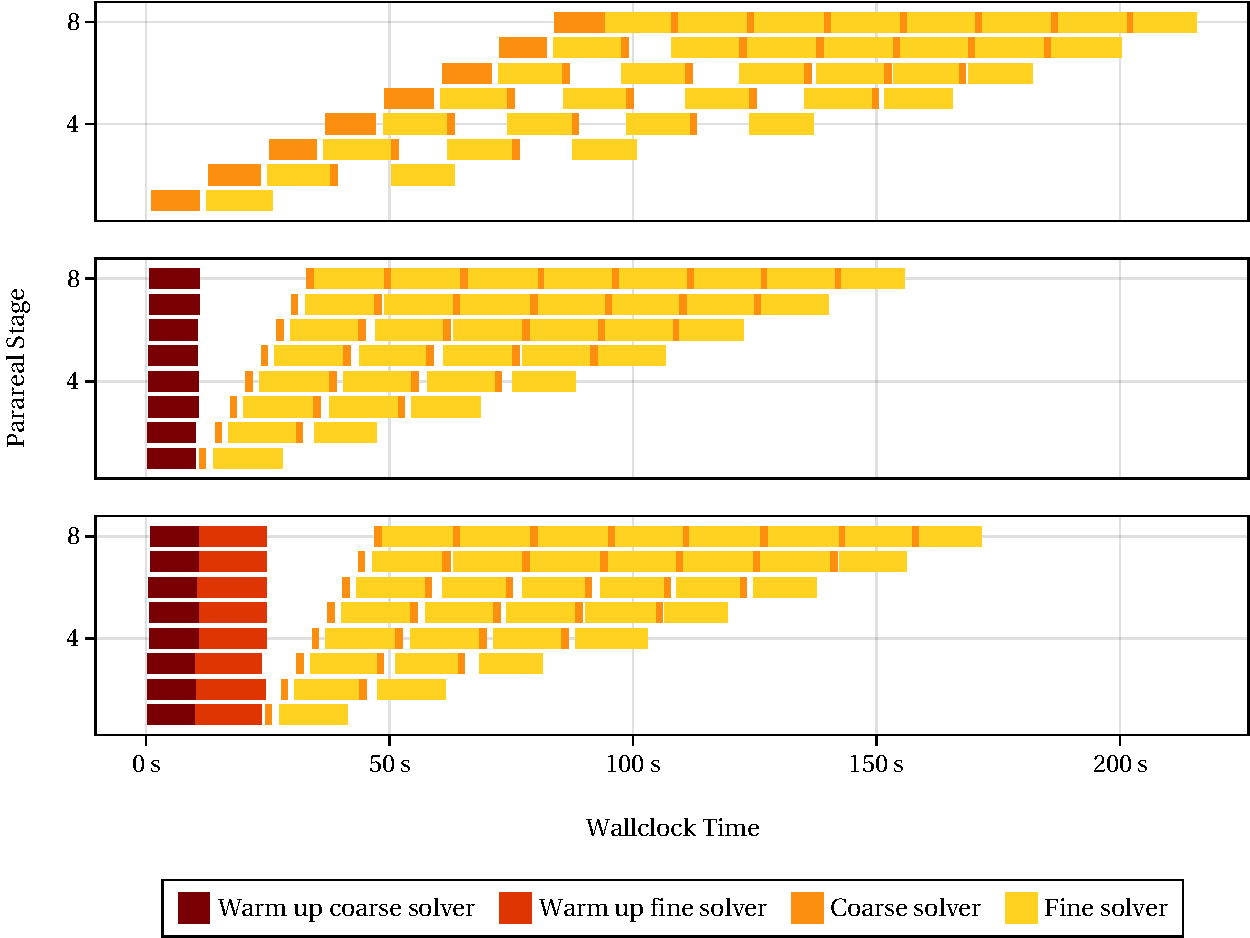
\includegraphics[width=\textwidth]{figures/fig_impl_warmup1.pdf}%
    \renewcommand\thefigure{7.1} % number in thesis
    \caption{Timeline charts\rlap{\hspace{3cm}%
    \lstinline!bash fig:impl:warmup.job!
    }}
    \end{figure}
  \column{0.35\textwidth}
    \begin{itemize}
      \item
        No warm-up:\\ sequential compilation
        \vspace{2.4em}
      \item
        Warming-up $G$:\\ parallel compilation
        \vspace{2.4em}
      \item
        Warming-up $F,G$:\\ no further benefit
        \vspace{2.4em}
      \pause
      \item[$\leadsto$]
        Always warm-up $G$\\ and $G$ only
    \end{itemize}
    \vspace{2em}
  \end{columns}
\end{frame}

\begin{frame}[t,label=runtime]{\secname}
  \framesubtitle{\subsecname}
  \begin{block}{Runtime Model}
  %\vspace{-\baselineskip} % maybe needed if in column
  \begin{equation*}
    \hattpar
    := \twarmup
    + \underbrace{
      \strut
      N \cdot (\trampup + t_G)
    }_{\substack{
      \text{stages $1\leq n\leq N$}\\
      \text{refinement $k=0$}
    }}
    + \underbrace{
      \strut
      K \cdot (t_F + t_G)
    }_{\substack{
      \vphantom{\text{stage}}
      n = N \\
      1 \leq k \leq K
    }}
    + t_F
  \end{equation*}
  \end{block}
  \only<1>{%
  \begin{columns}[onlytextwidth]
  \column{0.7\textwidth}
  \begin{figure}
    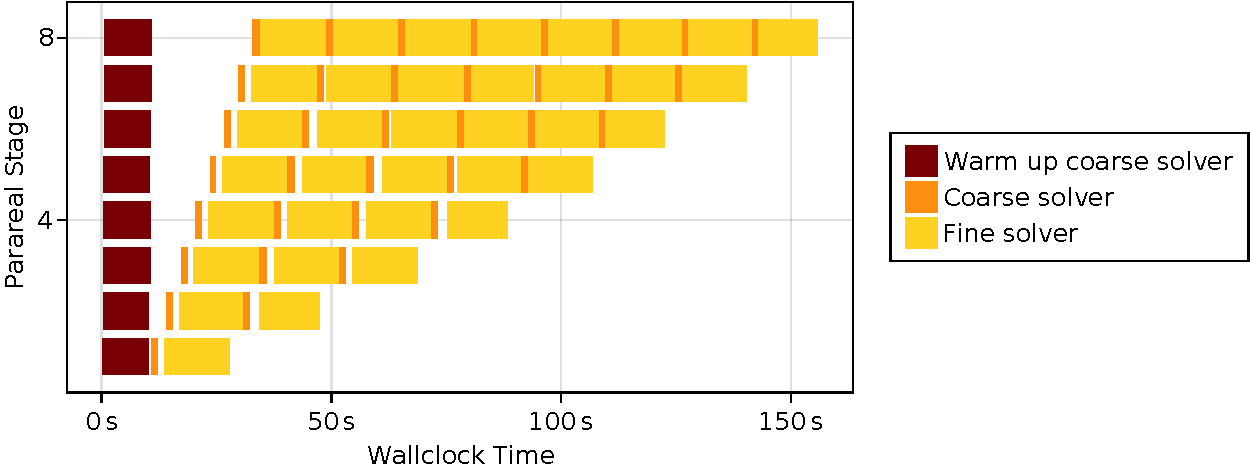
\includegraphics[width=0.95\textwidth]{figures/slides_timeline8.pdf}
    \caption{Timeline of $N=8$ stages computing $K=7$ refinements}
  \end{figure}
  \column{0.32\textwidth}
  \begin{itemize}
    \item under suitable assumptions
    \item $t_G/t_F$: runtime of coarse/fine solver
    \item $\twarmup$: duration of warm-up %TODO: is this really needed?
    \item $\trampup$: delay between first coarse solves
  \end{itemize}
  \end{columns}
  }
  \only<2>{%
  \setbeamertemplate{caption}[numbered]
  \vspace{-\baselineskip}
  \begin{table}
    \renewcommand\thetable{7.1} % number in thesis
    \caption{Runtime measurements for dense Rail371. (timings in seconds)}
    \small
    \begin{tabular}{%
      lcc
      S[table-format=2.2]
      S[table-format=2.2]
      S[table-format=1.2]
      S[table-format=2.2]
      S[table-format=3.2]
      S[table-format=3.2]
      S[round-precision=3, round-minimum=0.001, table-format=<1.3, scientific-notation=fixed, fixed-exponent=0] % err
    }
      \toprule
      {warm-up} &
      {$N$} &
      {$K$} &
      {$\twarmup$} &
      {$\trampup$} &
      {$t_G$} &
      {$t_F$} &
      {$\tpar$} &
      {$\hattpar$} &
      {$\abs*{\frac{\hattpar-\tpar}{\tpar}}$} \\
      \midrule
      none & 8 & 7 & 0.0 & 10.448182003838676 & 1.3971984386444092 & 13.686557531356812 & 215.85136604309082 & 214.03589286123002 & -0.008410756045427896 \\
$G$ & 8 & 7 & 10.995897054672241 & 1.7753152676991055 & 1.3795734643936157 & 14.053897976875305 & 155.979896068573 & 158.32320497717177 & 0.015023147005871765 \\
$G$ and $F$ & 8 & 7 & 24.658120155334473 & 1.805815781865801 & 1.3864995241165161 & 13.99841558933258 & 171.88022804260254 & 171.88946398666928 & 5.373476735471789e-5 \\

      \bottomrule
    \end{tabular}
  \end{table}
  \vspace{-\baselineskip}
  \begin{columns}[t,onlytextwidth]
  \column{0.285\textwidth}
  \begin{itemize}
    \setlength{\itemsep}{0pt}
    \item $\twarmup$: maximum
    \item $t_F,t_G$: median
  \end{itemize}
  \column{0.4\textwidth}
  \begin{itemize}
    \item $\trampup$: mean dealy between\\ first coarse solves minus $t_G$
  \end{itemize}
  \column{0.3\textwidth}
  \begin{itemize}
    \item actual runtime $\tpar$:\\ end of last fine solve
  \end{itemize}
  \end{columns}
  }
\end{frame}

